Decentralized systems are vulnerable to \textbf{Sybil attacks} in which an external attacker creates multiple fake identities in order to disrupt the normal behaviour of the network. This is an important issue especially in a system which needs to route messages between hosts, like the Distributed Hash Tables (DHT), since an attacker could prevent honest nodes to communicate.
Obviously, nodes cannot distinguish between an honest and a Sybil node, otherwise, the would simply reject the malicious entities.

Several solutions are available in order to strengthen the current protocols against this type of attacks: a central authority could provide certificates for discerning between honest and malicious nodes or unstructured protocols could be used which works by flooding or gossip. 
However, the cost of keeping universal identities could be too high. Moreover, protocols which work by flooding would require a linear time in order to find a specific key.

Whanau \cite{lesniewski2010whanau} is a novel protocol devised by Chris Lesniewski-Laas and M. Frans Kaashoek which provides an efficient solution to implement a DHT which is resistant to Sybil attacks. It has sub-linear run time and space usage. In order to reach this goal, Whanau exploits the properties of social networks such to build its network and it achieves these performances by combining the idea of \textbf{random walks} and a new way to construct the node's IDs called \textbf{layered identifiers}. Given $k$ keys and given the size of the network be $n$, the procedure build routing tables with $O(\sqrt{kn}\log(n))$ per node. Using Whanau's lookup tables, it is possible to show that a lookup provably takes $O(1)$ time. Moreover, Whanau's security does not impact the performance of the system. It scales similarly to other one-hop DHTs which provides no security.

In this work, we provided one of the first Java open-source implementations of Whanau by employing the Peersim \cite{montresor2009peersim} framework. We also conducted several experiments on synthetic networks such to replicate and validate the results obtained in the original paper. 

The following report is structured as follow. Section \ref{scenario} provides the scenarios to which Whanau was applied and tested. Section \ref{assumpt} shows the basic assumption on which Whanau's relies on in order to work correctly. 
Section \ref{struct} and Section \ref{prot} explains the details of the Whanau protocol such as how it builds its routing tables and how the lookup procedure work. Section \ref{impl} details how Whanau was implemented into the Peersim framework. Section \ref{exper} shows the results of the experiment we did in order to assess Whanau's function. Finally, in Section \ref{concl} we summarize our findings and we reason about eventual future works.

\section{Scenario\label{scenario}}
We applied Whanau to a simple Instant Messaging (IM) P2P application. Whanau provides the routing service for the clients. Each user is identified by a pair $(public\_key, ip\_address)$ which is saved inside the DHT. To send an IM to a specific user, we first need to look up its IP address by searching for his public key inside the DHT. Once the key is found, the client can connect directly to its target since it will know the target's IP address. Moreover, it would be possible to further complicate this application by including a validation procedure on the IP found, by checking if it was signed by the real user.  In our example, each node stores just one pair $(public\_key, ip\_address)$ but, in general, there may be $k>1$ per node. 

\section{Whanau's Assumptions\label{assumpt}}
Whanau relies on certain features of social networks in order to work properly. In this section, we will explain the two main assumptions that Whanau's make and why they are satisfied in a real-world scenario.

\subsection{Fast-mixing Social Networks}

A \textbf{social network} is an undirected graph in which a node knows its immediate neighbours. An \textbf{attack edge} is a connection between an honest node and a Sybil one.  An \textbf{honest edge} is a connection between two honest nodes.
Conceptually, we can divide a social network into two parts: a \textbf{Sybil region}, which is made by all the Sybil nodes/identities, and an \textbf{honest region}, which is comprised by all the honest nodes and their honest edges.

The key assumption is that the number of attack edges $g$ is relatively small with respect to the honest nodes $n$ ($g \ll n$). This means that it exists a \textbf{sparse cut} between the honest region and the Sybil region (Figure \ref{fig:sparse_cut} shows an example of sparse cut). This assumption can be justified because, in order to add a new attack edge, a Sybil node must do a social-engineering effort: an attacker must convince an honest person to create a social link to one of the Sybil identities.

Given these assumptions, the honest region forms an \textbf{expander graph}. Expander graphs are \textbf{fast mixing}, which means that the ending node of a random walk is a random node in the network, with a probability distribution proportional to the node's degree. We can then define the \textbf{mixing time}, $w$, which is the number of steps required in order to reach this kind of distribution. For a fast mixing graph, $w = O(\log(n))$.

\subsection{Sampling by Random Walks}

The \textbf{random walk} is the main building block of Whanau and it is the only way the protocol has to use the social network. Given the previous assumptions, an honest node can send around several $w$-random walks in order to sample nodes from the network ($w$-random walks means that the length of the path will be equal to the mixing time $w$). If the social network is fast-mixing and if it has a sparse cut, the resulting set of sampled nodes will contain several honest nodes and few Sybil nodes, since we will have a much higher probability of ``avoiding" the Sybil region.
Some nodes will be close to many attack edges, those are called \textbf{looser nodes} since they were too relaxed when making social connections. 
They will need to use more lookup messages in order to escape the Sybil region, thus wasting more bandwidth. Fortunately, the number of looser nodes in a network will be small (thanks to the sparse cut assumption) and most nodes will be \textbf{winner nodes}.

\begin{figure}[h]
    \centering
    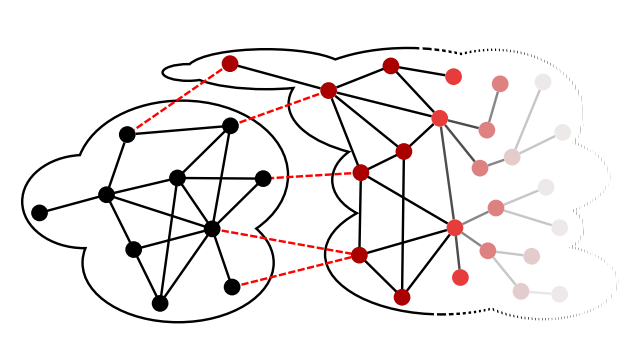
\includegraphics[width=\linewidth]{sparse_cut.png}
    \caption{An example of a sparse cut in a social network. The dashed connections are the attack edges. Black nodes are honest nodes. Red nodes are the Sybil ones.}
    \label{fig:sparse_cut}
\end{figure}

\section{Whanau's Structure \label{struct}}

\subsection{General Working Principle}

In the bootstrapping phase, each node performs $r=O(\sqrt{km})$ independent $w$-random walks on the social network. It then collects a random $(key, value)$ record for each final nodes and stores these nodes and record in a local table.

In order to perform a lookup operation, a node $u$ checks its local record table. If the key is not in the table, $u$ broadcast the target key to the nodes in its local table (which were sampled before). If the table size is sufficiently large, at least one node $v_i$ will have the needed key in its local table. 

This procedure will mitigate the presence of Sybil nodes. If the number of attack edges is small, the nodes will mostly sample from the honest region. Thus, the local tables will contain mostly honest nodes/records. Moreover, nodes do not look to each other tables during the setup process. Therefore the attacker influence does not increase over time.

However, this first draft of the protocol does not take into account the nodes IDs, therefore limiting its efficiency (it is basically broadcasting many messages wasting CPU and bandwidth) and it is still vulnerable to clustering attacks. Therefore, the next sections will be devoted to providing an explanation about the structures used by Whanau in order to be efficient and clustering-resistant.

\subsection{No metric space} Whanau does not embed the keys into a metric space by using a hash function (as some other DHT like Chord \cite{stoica2001chord} or Kademlia \cite{maymounkov2002kademlia}) since the adversary could guess-and-check and craft many keys that fall between any two neighbouring honest node keys. Therefore, Whanau does not have any notion of ``distance" between keys. However, it does assume a \textbf{global circular ordering} on keys, such to be able to determine if one key falls between two other keys (this however still requires defences to clustering attacks). This way nodes will able to build a successor's table. 

\subsection{Fingers and Successors} Many structured DHT have tables which contain ``far pointers" (fingers) and successors. Whanau follows this pattern. All node have layered IDs which are of the same data type as the key. Moreover, each node has the following tables:
\begin{itemize}
    \item \textbf{Finger Table}: it contains ($O(\sqrt{km})$) pointers to other nodes which are spaced evenly over the key space;
    \item \textbf{Successor Table}: it contains ($O(\sqrt{km})$) pointers to honest $(key,value)$ record which immediately follow the node ID. 
\end{itemize}
This tables are built by sampling the nodes by sending out $O(\sqrt{km})$ $w$-random walks on the network (the successor table is actually built with a more complex sampling procedure).

The most important point is that this table architecture enables fast one-hop lookups. If a node wants to search for a key, it will first look at its own successor table to see if it has already the needed value. If this does not succeed, it will send a query message to a finger node preceding the target key. It is possible to prove that this target node will have with high probability the needed value in its own successor table if it is honest.

\begin{figure}[t]
    \centering
    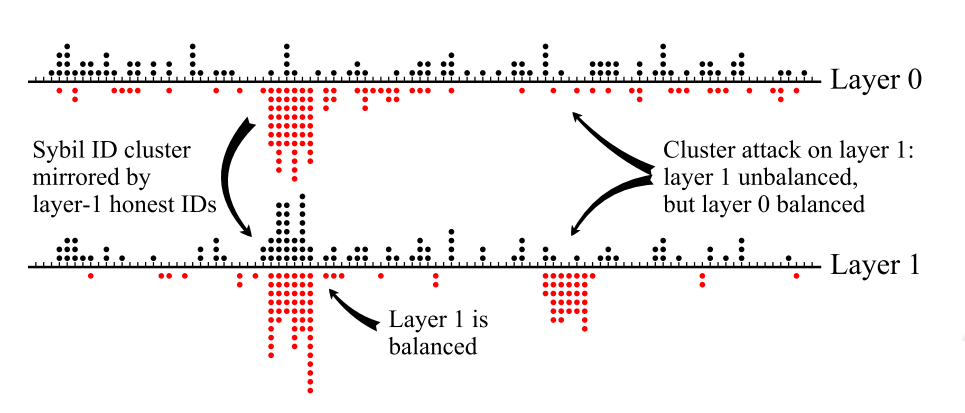
\includegraphics[width=\linewidth]{layers.png}
    \caption{Black dots represent honest nodes, while red dots represent Sybil nodes. The figures shows how Whanau deal with clustering attacks. Even if the layer-0 IDs are unbalanced, the honest nodes will ``cluster" around the target key inside layer-1 IDs, thus enabling other nodes to find that key regardless of the Sybil nodes.}
    \label{fig:layers}
\end{figure}

\subsection{Layered IDs}
Whanau uses layers to defend against clustering attacks. Each node uses a $w$-random walk to choose a random key as its own layer-0 ID. In order to pick a layer-1 ID, each node picks a random entry from its own layer-0 finger table and uses that node's ID. To pick a layer-2 ID we sample from the layer-1 finger table and so on an so forth for all the $l = O(\log(km))$ layers.  

If an attacker were to craft all its identities (IDs) to fall near a target key on layer-0, this will just cause all the other honest nodes to choose an ID in that range as their layer-1 ID (this will propagate also over all the subsequent layers).  This increases the presence of honest nodes in the adversary range, thus making more likely to find the target key which is affected by the clustering attack. 

\section{The Whanau Protocol \label{prot}}

\begin{figure}[h]
    \centering
    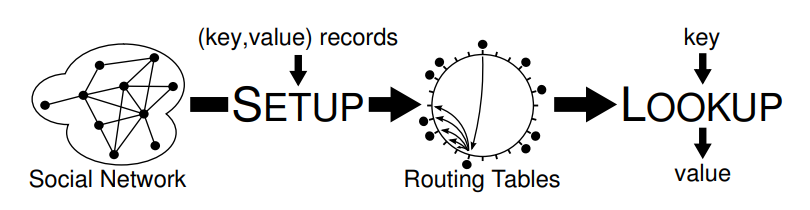
\includegraphics[width=\linewidth]{whanau.png}
    \caption{The Whanau Protocol}
    \label{fig:whanau_protocol}
\end{figure}

The Whanau protocol is made by only two procedures, \textsc{setup} and \textsc{lookup}. The former is used to initialize the DHT from the social network and it is run periodically in order to deal with network churn. The latter is used to find the target key. Figure \ref{fig:whanau_protocol} shows a visual overview of the entire process.

\subsection{\textsc{Setup} procedure}
\begin{algorithm} % enter the algorithm environment
\caption{Whanau's \textsc{setup} procedure} % give the algorithm a caption
\label{alg:setup} % and a label for \ref{} commands later in the document
\begin{algorithmic}[1] % enter the algorithmic environment
    \FOR{ each node $u$}
        \STATE $db(u) \gets $\textsc{SAMPLE-RECORDS}($u$, $r_d$)
    \ENDFOR
    \FOR{$i \gets 0 $ to $l$}
        \FOR{each node $u$}
            \STATE $ids(u, i) \gets$ \textsc{CHOOSE-ID}$(u,i)$
            \STATE $fingers(u, i) \gets$ \textsc{FINGERS}$(u,i, r_f)$
            \STATE $successors(u, i) \gets$ \textsc{SUCCESSORS}$(u,i, r_s)$
        \ENDFOR
    \ENDFOR
\end{algorithmic}
\end{algorithm}

The \textsc{setup} procedure takes the social network connections, the local key value records and build for each nodes four tables:
\begin{itemize}
    \item \textit{ids(u,i)}: it contains, for each layer $i$, the node's ID; 
    \item \textit{fingers(u,i)}: it contains, for each layer $i$, pointers to the node fingers;
    \item \textit{successors(u,i)}: it contains, for each layer $i$, key-value records contained in the successor nodes;
    \item \textit{db(u)}: a sample of records which is used to construct \textit{successors};
\end{itemize}
Pseudocode \ref{alg:setup} shows the steps done by \textsc{setup}. The procedure takes also some additional parameters $r_d$, $r_f$, $r_s$ which specify the size of the routing tables (how many samples we need to take). A detailed explanation of all the additional methods used can be found on the original paper.

The \textsc{setup} procedure ensure that any honest finger $f$ which is ``close enough" to the target key $y$ will have $y \in successors(f)$.


\textsc{setup} is an iterative procedure that builds up the routing tables layer after layer starting from the first one (\textit{layer, 0}). As previously described, the \textit{layer-0} ID is sampled from the stored keys $db(u)$, on the node (which were sampled by random walk). Fingers (and successors) are values are then sampled by a random walk of the graph. From layer 1 to \textit{l} the procedure picks:
\begin{itemize}
    \item \textit{id} : the \textsc{choose-finger} method picks one of the fingers of the previous layers (effectively shuffling the keys based on random walks). This ``reshapes" the distribution of the keys to match the one in the previous layer, thus contrasting clustering attack on certain keys (see Fig. \ref{fig:key_distributions} for an example of key distribution under a clustering attack);
    \item \textit{fingers} : the \textsc{fingers} methods re-samples new nodes for the current layer  with random walks;
    \item \textit{successors} : the \textsc{successors} method works in the same fashion as for the \textsc{fingers} one, but instead sampling keys, it samples successors from the ending nodes of the random walks.
\end{itemize}

\begin{figure*}[t]
    \centering
    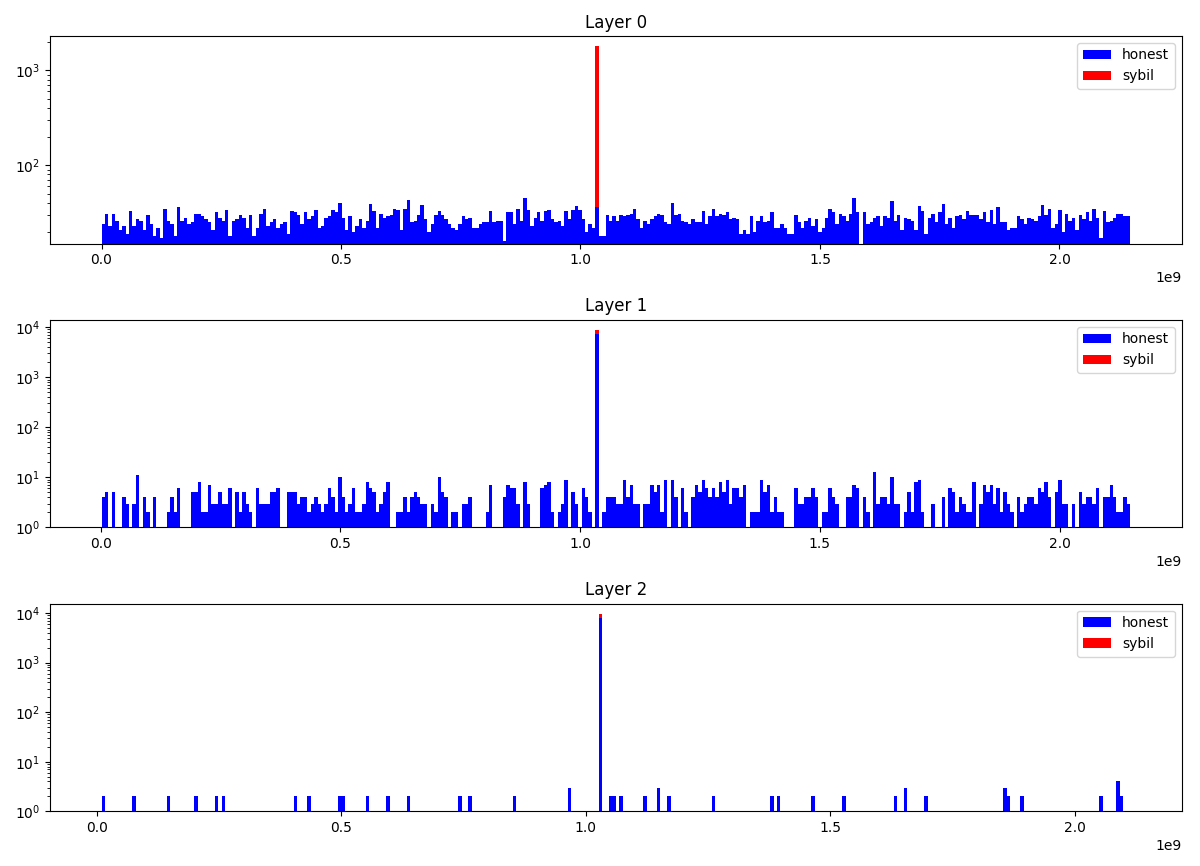
\includegraphics[scale=0.4]{keys2.png}
    \caption{Example of the distribution of the keys (integers in $[0,2^{31}-1]$, grouped in 300 bins) in the $ids$ node's tables built on a synthetic network. The y-axis is in logarithmic scale. \textit{Layer}-0 shows the presence of a clustering attack: $\approx1100$ nodes out of the $10^4$ are Sybil and chose their $layer$-0 key near the one they want to attack. In subsequent layers ($layers$-1 and $layers$-2) it is clear that with the key sampling procedure, the honest node overcame the high concentration of malicious nodes around the key of interest, thus reducing the effect of the clustering attack.}
    \label{fig:key_distributions}
\end{figure*}



\subsection{\textsc{Lookup} procedure}

\begin{algorithm} % enter the algorithm environment
\caption{Whanau's \textsc{lookup} procedure} % give the algorithm a caption
\label{alg:lookup} % and a label for \ref{} commands later in the document
\begin{algorithmic}[1] % enter the algorithmic environment
    \STATE $value \gets null; v \gets u$
    \REPEAT
        \STATE $value \gets$ \textsc{TRY}$(v, key)$
        \STATE $v \gets$ \textsc{RANDOM-WALK}$(u)$
    \UNTIL{\textsc{TRY} found a valid $value$, or hit retry limit}
    \RETURN $value$
\end{algorithmic}
\end{algorithm}

The objective of the \textsc{lookup} procedure is to find a finger node $f$ which is honest and such that it has the target key in its \textit{successor} table. Pseudocode \ref{alg:lookup} shows the step executed. \textsc{Lookup} first tries using its own finger table, then, if the search has failed, it selects a random delegate and retries the search from there (until we reach a retry limit). The \textsc{try} procedure searches the finger table for the closest layer-0 ID $x_0$ to the target $key$. It then selects a random layer $i$ and a random layer-$i$ finger $f$ whose ID lies between $x_0$ and the $key$. \textsc{try} then queries $f$ for the target key.

It can be proved that there is a high probability that the \textsc{try} procedure will select an honest finger $f$ which will have $key \in successors(f)$. In conclusion, \textsc{lookup} should always succeed after only a few calls to \textsc{try}.  

\subsection{Network Churn}
\textbf{Churn} refers to a change in the availability of nodes or keys in the system (i.e. new nodes join/leave the network and/or new keys are added/deleted from the DHT).

\textbf{Node churn} is not an issue: the original paper states that temporary unavailability of nodes (e.g. due to network failures such as latencies) is not a problem and it results in small delays in the retrieval of the wanted key(s). These results come from simulations on \textbf{PlanetLab} (1353 nodes). However, as the original authors noted,  these conclusions cannot be inductively extended to bigger networks due to lack of empirical experiments.

As a matter of fact, once initialised, the structure of the network is rather \textbf{static}: new nodes that joined after the setup stage and/or nodes leaving may result in inefficiencies for the protocol. A simple re-run of the \textsc{WhanauSetup} protocol fixes this issues. This can be safely done with a small overhead in with a repetition timeout in the order of minutes/hours. The optimal solution to this problem may differ from application to application and different approaches may perform better w.r.t. other in certain contexts.

\textbf{Key churn} is handled in the same way as we deal with addition/deletion of nodes, by repeatedly running the \textsc{setup} procedure after certain time intervals. Key churn (and no re-assessment with \textsc{setup}) may cause unbalanced \textit{successors} tables and create ``hotspots". This can result in network ID distributions on the nodes that do not resemble the actual updated distribution of keys.